\hypersetup{
    colorlinks=true,
    linkcolor=verdeApagado!80!black,
    filecolor=verdeApagado!80!black,      
    urlcolor=azulPastelApagado!80!black,
    pdftitle={Manual de Coordinación y Plan de Dirección}
}

\setlist[itemize]{leftmargin=1.5em, itemsep=3pt, topsep=3pt}
\setlist[enumerate]{leftmargin=1.5em, itemsep=3pt, topsep=3pt}

\section{Manual de Coordinación / Plan de Dirección}

\begin{small}
\textit{Este documento debe ser completado, aprobado y firmado por todos los implicados en la gestión y desarrollo del proyecto.}
\end{small}

\vspace{0.5em}

% -----------------------------------------------------------------
% METODOLOGÍA
% -----------------------------------------------------------------
\subsection{Metodología de Desarrollo y Ciclo de Vida}

La metodología de desarrollo elegida es Scrum, ya que permite organizar el trabajo en periodos cortos, establecer objetivos concretos y adaptar la aplicación a partir de las revisiones realizadas durante su desarrollo.

El proyecto se organizará en una fase inicial de preparación y en tres iteraciones de desarrollo:

\begin{itemize}
    \item \textbf{Fase inicial (iteración 0):} Se abordará el análisis de los requisitos iniciales, la realización del manual de coordinación, de la propuesta técnica del proyecto y del registro de horas y actas de reuniones.
    \item \textbf{Iteración 1, Iteración 2, Iteración 3.}
\end{itemize}

Al comienzo de cada iteración se establecerán los objetivos y las tareas previstas, así como la organización del equipo, y al finalizar, se revisará el trabajo realizado, se identificarán las tareas pendientes y se recogerán propuestas de mejora para la siguiente iteración.

% -----------------------------------------------------------------
% RECURSOS SOFTWARE
% -----------------------------------------------------------------
\subsection{Recursos Software Desarrollo}

Las herramientas, lenguajes y tecnologías previstos para el desarrollo son los siguientes:

\begin{table}[htbp]
\centering
\small
\rowcolors{2}{white}{azulclaro!50}
\begin{tabularx}{\textwidth}{l l X}
\toprule
\rowcolor{azulPastelApagado}
\textbf{Categoría} & \textbf{Tecnología} & \textbf{Propósito / Función} \\
\midrule
Front-end & HTML & Estructuración del contenido de las páginas web. \\
          & CSS & Definición de los estilos y la presentación visual de la aplicación. \\
          & JavaScript & Implementación de funcionalidades. \\
Back-end  & PHP & Desarrollo de la lógica del servidor. Se encargará de procesar las peticiones de los usuarios, gestionar la información recibida, comunicarse con la base de datos MySQL y generar las respuestas que se mostrarán en la interfaz web. \\
          & MySQL & Almacenamiento y gestión de los datos de la aplicación. \\
Infraestructura & Docker & Configuración y ejecución de los servicios necesarios en contenedores separados. \\
Gestión y Control & Git y GitHub & Control de versiones y almacenamiento compartido del código fuente. \\
                  & Jira & Planificación, asignación y seguimiento de las tareas del proyecto. \\
                  & \LaTeX & Elaboración de la documentación siguiendo un formato común. \\
Comunicación & Discord y/o WhatsApp & Comunicación interna del equipo. \\
\bottomrule
\end{tabularx}
\caption{Recursos software y tecnologías previstos para el proyecto.}
\label{tab:recursos_software}
\end{table}

% -----------------------------------------------------------------
% ORGANIZACIÓN DEL EQUIPO
% -----------------------------------------------------------------
\subsection{Organización del Equipo de Trabajo (Estructura, Normas)}

La organización administrativa del equipo se distribuirá en una asignación de roles fija para los siguientes cargos:

\begin{table}[htbp]
\centering
\small
\rowcolors{2}{white}{azulclaro!50}
\begin{tabularx}{\textwidth}{l X}
\toprule
\rowcolor{verdeApagado}
\textbf{Cargo Fijo} & \textbf{Integrante Asignado} \\
\midrule
Catalogador & Cristina García Gázquez. \\
Moderador & Ángela García Olmos. \\
Presentador & Daniel Vega Jiménez. \\
Gestor de Calidad & Minerva Cebrián Marín. \\
Gestor de Usabilidad y Accesibilidad & Pedro Javier Pérez Jiménez. \\
\bottomrule
\end{tabularx}
\caption{Asignación fija de roles administrativos.}
\label{tab:roles_fijos}
\end{table}

Y, una asignación variable para el cargo de coordinador, el cual se distribuirá de la siguiente forma:
\begin{itemize}
    \item \textbf{Iteración 0:} Daniel Vega Jiménez.
    \item \textbf{Iteración 1:} Minerva Cebrián Marín.
    \item \textbf{Iteración 2:} Pedro Javier Pérez Jiménez.
    \item \textbf{Iteración 3:} Cristina García Gázquez y Ángela García Olmos.
\end{itemize}

Las responsabilidades de cada rol serán las siguientes:

\begin{itemize}
    \item \textbf{Coordinador:} Organizar el trabajo de la iteración, comprobar el estado general de las tareas, facilitar la resolución de bloqueos y coordinar la preparación de las reuniones.
    \item \textbf{Catalogador:} Mantener organizada y actualizada la documentación del proyecto, facilitar su localización y comprobar que los documentos se encuentren en las ubicaciones acordadas.
    \item \textbf{Moderador:} Facilitar la participación de todos los integrantes en las reuniones, mantener el orden del debate y ayudar a alcanzar acuerdos.
    \item \textbf{Presentador:} Coordinar la preparación de las presentaciones y organizar la exposición del proyecto, contando con la participación del resto del equipo.
    \item \textbf{Gestor de Calidad:} Definir y supervisar los criterios de calidad, comprobar que se realizan las revisiones y pruebas acordadas y registrar los errores detectados.
    \item \textbf{Gestor de Usabilidad y Accesibilidad:} Supervisar que las decisiones de diseño e implementación tengan en cuenta las necesidades de los usuarios, la facilidad de uso y los requisitos de accesibilidad.
\end{itemize}

En cuanto a la organización técnica del equipo, todos los integrantes podrán participar en las diferentes tareas del proyecto. No obstante, se establece la siguiente asignación para facilitar el reparto inicial del trabajo:

\begin{itemize}
    \item \textbf{Front-end:} Cristina García Gázquez, Ángela García Olmos.
    \item \textbf{Back-end:} Daniel Vega Jiménez, Pedro Javier Pérez Jiménez, Minerva Cebrián Marín.
\end{itemize}

Esta distribución no será exclusiva. El equipo podrá modificarla según las necesidades de cada iteración, la carga de trabajo y las competencias de los integrantes.

Daniel Vega Jiménez coordinará la preparación y organización de las entregas y el resto del equipo deberá revisar los documentos y la aplicación antes de su presentación.

Las normas de funcionamiento generales del equipo serán las siguientes:

\begin{enumerate}
    \item Consultar las dudas antes de tomar decisiones basadas en suposiciones.
    \item Comprobar en Jira si una tarea ya está asignada o en desarrollo antes de comenzar a trabajar en ella.
    \item Compartir los avances y poner en común los resultados, especialmente antes de realizar una entrega.
    \item Tomar las decisiones por consenso siempre que sea posible. Si no se alcanza un acuerdo, se recurrirá a una votación por mayoría.
    \item Respetar los plazos acordados y avisar con antelación cuando exista riesgo de retraso.
    \item Comunicar los bloqueos y solicitar ayuda cuando sea necesario.
    \item Revisar las aportaciones del resto del equipo de forma constructiva, ayudando a la resolución de problemas.
    \item Distribuir el trabajo de forma equilibrada, teniendo en cuenta la dificultad de las tareas, el tiempo disponible, las responsabilidades asumidas y el trabajo realizado en iteraciones anteriores.
    \item Dejar constancia de los acuerdos y decisiones relevantes en las actas de reunión.
\end{enumerate}

% -----------------------------------------------------------------
% COMUNICACIÓN Y CLIENTE
% -----------------------------------------------------------------
\subsection{Herramientas para Comunicaciones en el Equipo de Trabajo}

La comunicación interna se realizará principalmente mediante Discord y/o WhatsApp, dependiendo del requerimiento en ese momento.
\begin{figure}[htbp]
    \centering
    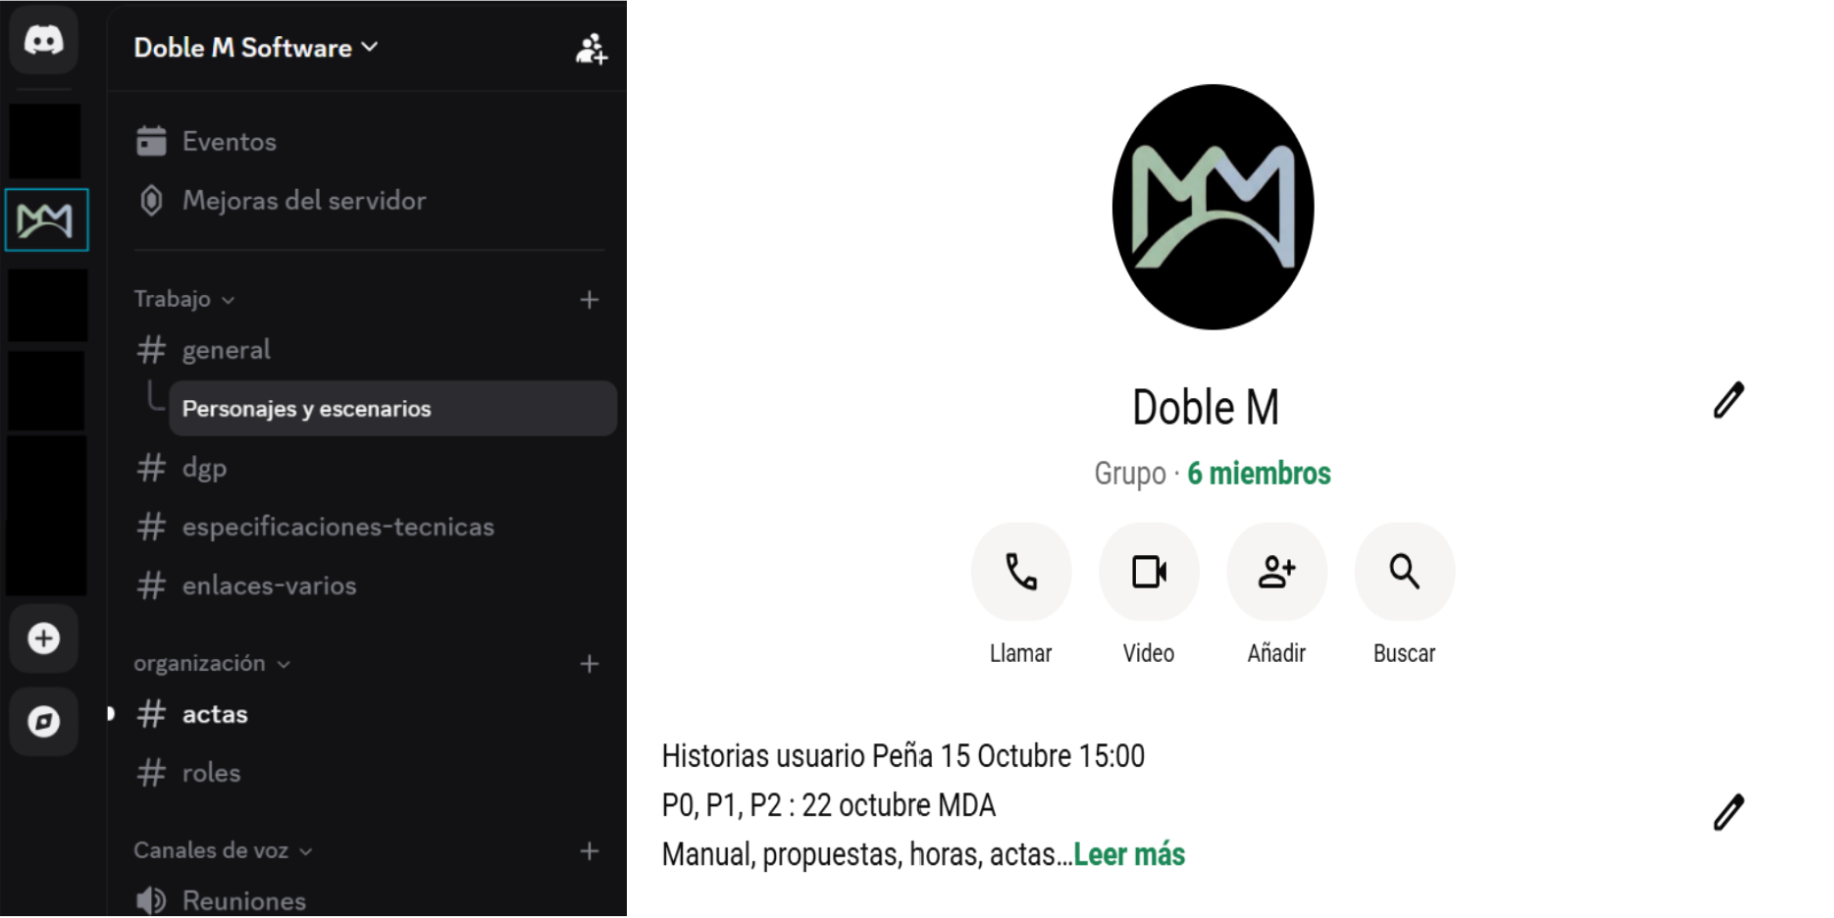
\includegraphics[width=0.8\textwidth]{img/grupo_comunicacion.png}
    \caption{Foto del grupo de WhatsApp y Discord del equipo de trabajo.}
    \label{fig:grupo_comunicacion}
\end{figure}

Estas herramientas se emplearán para resolver dudas rápidas, comunicar incidencias, coordinar reuniones y avisar de cambios que puedan afectar al trabajo de los demás integrantes.

Las reuniones de coordinación servirán para revisar el estado de las tareas, identificar bloqueos, acordar prioridades y organizar el trabajo pendiente.

Además, para tener un seguimiento de los documentos y los elementos básicos para la coordinación y estandarización de los documentos, empleamos GitHub.
\begin{figure}[htbp]
    \centering
    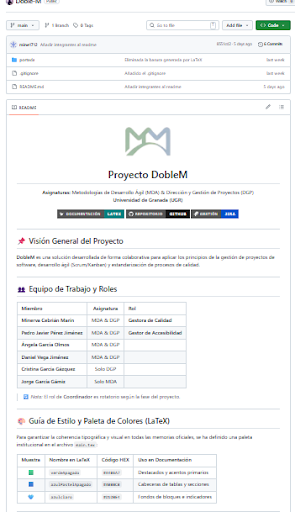
\includegraphics[width=0.8\textwidth]{img/github.png}
    \caption{Foto del repositorio de Github.}
    \label{fig:repo_github}
\end{figure}


\subsection{Relaciones con el Cliente (Entrevistas, Reuniones, Revisiones, \dots)}

La relación con el cliente y con el profesorado se establecerá mediante entrevistas, reuniones de seguimiento y comunicaciones por correo electrónico, para formular consultas concretas o enviar alguna información.

Después de cada reunión o entrevista, se recogerán los aspectos tratados, los acuerdos alcanzados, y las dudas pendientes y cuando sea necesario, se actualizarán los requisitos y las tareas a realizar.

Los cambios solicitados por el cliente se evaluarán teniendo en cuenta su prioridad, su impacto sobre las funcionalidades existentes, el esfuerzo necesario y los plazos de entrega.

% -----------------------------------------------------------------
% ESTÁNDARES
% -----------------------------------------------------------------
\subsection{Estándares de Documentación}

La documentación del proyecto se elaborará utilizando \LaTeX, con el objetivo de mantener un formato uniforme y facilitar su revisión y mantenimiento, siguiendo las siguientes normas:

\begin{itemize}
    \item Los documentos tendrán una portada común con el nombre del equipo y logo, las asignaturas, los integrantes del equipo y la fecha.
    \item Se utilizarán los colores corporativos establecidos.
    \item Se empleará una estructura común de títulos, apartados, tablas, figuras y referencias.
    \item Los archivos fuente se conservarán en formato .tex y las versiones finales se generarán en PDF.
    \item Las figuras y capturas tendrán un título o pie explicativo y se numerarán cuando corresponda.
    \item Se utilizará un lenguaje claro, preciso y coherente en todos los documentos.
    \item Los documentos se guardarán en las carpetas acordadas y se mantendrá un control de sus versiones.
\end{itemize}

\subsection{Estándares de Código}

El código del proyecto seguirá unos estándares comunes para facilitar su lectura, mantenimiento y revisión por parte de todos los integrantes, donde se aplicarán las siguientes normas:

\begin{itemize}
    \item Los comentarios explicativos del código se escribirán en español, mientras que los nombres de variables, funciones, clases y otros identificadores se escribirán en inglés.
    \item Las variables y funciones utilizarán el formato \texttt{camelCase}.
    \item Las clases utilizarán el formato \texttt{PascalCase}.
    \item Las constantes utilizarán el formato \texttt{UPPER\_SNAKE\_CASE}.
    \item Cada función tendrá una responsabilidad concreta y se evitarán funciones excesivamente largas o con demasiadas responsabilidades.
    \item Se evitará duplicar código mediante la reutilización de funciones, siempre que sea posible.
    \item Se utilizarán nombres descriptivos que permitan comprender la finalidad de las variables y funciones.
    \item Se evitará introducir cambios que no estén relacionados con la tarea asignada, salvo que sean necesarios y se comuniquen al equipo.
\end{itemize}

Cuando se incorporen nuevas funcionalidades o se modifique código existente, se realizarán las pruebas que correspondan. Los errores detectados deberán corregirse o registrarse como tareas pendientes en Jira.

% -----------------------------------------------------------------
% GESTIÓN DE CAMBIOS Y CONTROL DE VERSIONES
% -----------------------------------------------------------------
\subsection{Plan de Gestión de Cambios}

Cualquier cambio que afecte a los requisitos, las funcionalidades, el diseño, la planificación o la tecnología deberá comunicarse a todo el equipo y el procedimiento a seguir será el siguiente:

\begin{enumerate}
    \item Se describirá el cambio solicitado o la necesidad detectada.
    \item Se analizará su prioridad y el esfuerzo necesario que requerirá sobre el trabajo ya realizado.
    \item El equipo determinará si el cambio se incorpora a la iteración actual, se planifica para una iteración posterior o se descarta justificadamente.
    \item Si se acepta, se modificarán los requisitos, las tareas, la planificación y la documentación afectada.
    \item Se comprobará que la modificación funciona correctamente y que no ha perjudicado a otras funcionalidades.
\end{enumerate}

Si un integrante no puede completar una tarea asignada, deberá comunicarlo lo antes posible. El equipo valorará la posibilidad de prestar apoyo, reasignar la tarea o dividirla en partes más pequeñas, procurando mantener una distribución equilibrada del trabajo.

\subsection{Control de Versiones (Método y Herramientas)}

El control de versiones se realizará mediante Git y GitHub. El repositorio contendrá el código fuente y los archivos de configuración y documentación.

% -----------------------------------------------------------------
% CALIDAD, DESEMPEÑO Y RECOMPENSAS
% -----------------------------------------------------------------
\subsection{Gestión de Calidad (Durante el Desarrollo y al Final, Incluir Herramientas)}

La gestión de la calidad se realizará durante todo el desarrollo y no únicamente al finalizar el proyecto. Su objetivo será comprobar que el producto cumple los requisitos acordados, que funciona correctamente y que la documentación es coherente con la implementación.

Se llevarán a cabo las siguientes actividades:

\begin{itemize}
    \item Comprobar que las funcionalidades implementadas corresponden con los requisitos e historias de usuario acordados.
    \item Utilizar Jira para comprobar el estado de las tareas, detectar retrasos e identificar trabajo pendiente.
    \item Comprobar la legibilidad, la coherencia con los estándares establecidos y la ausencia de errores.
    \item Verificar que las funcionalidades principales se comportan como se espera.
    \item Verificar que los documentos estén actualizados y tengan un formato común.
    \item Registrar los errores detectados, asignarles prioridad y comprobar su resolución.
\end{itemize}

El Gestor de Calidad coordinará estas actividades y registrará las incidencias relevantes. No obstante, todos los integrantes serán responsables de revisar la calidad de su propio trabajo y de colaborar en las comprobaciones comunes.

\subsection{Plan de Medición del Desempeño, Recompensas}

El seguimiento del desempeño se basará en criterios objetivos relacionados con el trabajo realizado, el cumplimiento de los compromisos y la colaboración con el equipo.

Si un integrante tiene dificultades para completar su trabajo, el equipo analizará las causas y acordará medidas de apoyo o una redistribución de tareas. Si se detecta un incumplimiento reiterado sin comunicación ni justificación, se hablará con la persona implicada y se documentarán los acuerdos de mejora. Si el problema persiste, se informará al profesorado.

Cuando un integrante asuma una carga de trabajo superior a la prevista, se tendrá en cuenta en la planificación posterior para procurar un reparto equilibrado y evitar la sobrecarga.

Como incentivo colectivo, el equipo propone celebrar el logro de una calificación de sobresaliente mediante una actividad de ocio acordada por todos los miembros, como una visita a un parque de atracciones o a un centro recreativo.